\chapter{Referencial Teórico}
Este capítulo apresenta um revisão teórica sobre as principais metodologias utilizadas nesse trabalho: programação linear, métodos de classificação e métodos de validação. Também é apresentada uma revisão de trabalhos sobre classificação de padrões.  

\section{A programação linear}
Na pesquisa operacional, a programação linear é uma das técnicas mais utilizadas para resolver problemas de otimização. Os problemas de programação linear geralmente buscam a distribuição eficiente de recursos limitados para atender um determinado objetivo, por isso suas aplicações estão presentes em diversas áreas como computação, administração, indústria e transporte \cite{Engecom}.

Um problema de programação linear é expresso através de um modelo composto por equações e inequações lineares. Esse tipo de problema busca a distribuição eficiente de recursos com restrições para alcançar um objetivo, em geral, maximizar lucros ou minimizar custos. Em um problema de programação linear esse objetivo é expresso através de uma equação linear denominada função objetivo. Para a formulação do problema, é necessário também definir os recursos necessários e em que proporção são requeridos. Essas informações são expressas em equações ou inequações lineares, uma para cada recurso. Esse conjunto de equações ou inequações é denominado restrições do modelo \cite{Engecom}.

\section{Descrição do Problema de Programação Linear}
O modelo de um problema de programação linear é apresentado em uma das formas a seguir:
\newpage
\noindent
\underline{\bf Modelo 1}
\begin{eqnarray}
    Max\ z = c^{T}x \label{eq:obj1}
\\s.a.\left\{\begin{matrix}
Ax\leq b\\*x\geq 0
\end{matrix}\right.\label{eq:rest1}
\end{eqnarray}
\\
\noindent
\underline{\bf Modelo 2}
\begin{eqnarray}
Min\ z = c^{T}x \label{eq:obj2}
\\*s.a.\left\{\begin{matrix}
Ax\geq  b\\*x\geq 0 
\end{matrix}\right. \label{eq:rest2}
\end{eqnarray}

Nos Modelos 1 e 2 as equações \ref{eq:obj1} e \ref{eq:obj2} representam as funções objetivo e as inequações \ref{eq:rest1} e \ref{eq:rest2} representam as restrições.
Onde, 
\begin{itemize}
\item \textbf {$x$} é o vetor com as variáveis do modelo
\item \textbf {$c$} é o vetor de coeficientes da função objetivo
\item \textbf {$z$} é o valor da função objetivo
\item \textbf {$A$} é a matriz com as constantes das restrições
\item \textbf {$b$} é o vetor com os valores limites das restrições
\end{itemize}

Sendo que c, A e b são dados conhecidos.

A seguir é apresentado um exemplo de aplicação da programação linear no contexto da otimização da produção. Uma empresa, que fabrica vários produtos, deseja maximizar o lucro na venda de dois desses produtos.
A produção é feita em três setores diferentes e está sujeita a restrições de tempo disponível para a produção em cada setor.
O problema pode ser representado pelo seguinte modelo de programação linear com duas variáveis\cite{Hillier}.

\begin{eqnarray}
Maximize\ z=3x_{1}+5x_{2}\label{eq2:eq1}\\ 
Sujeito\ a \nonumber \\ 
1x_{1}\leq 4 \label{eq2:eq2} \\  
2x_{2}\leq 12 \label{eq2:eq3} \\ 
3x_{1}+2x_{2}\leq 18 \label{eq2:eq4}\\ 
x_{1}\geq 0, x_{2}\geq 0 \label{eq2:eq5}
\end{eqnarray}

Onde, 
\begin{itemize}
\item \textbf {$x_{1}$} representa a quantidade do produto 1 produzido em uma semana.
\item \textbf {$x_{2}$} representa a quantidade do produto 2 produzido em uma semana.
\item \textbf {$z$} representa o lucro total por semana de produção desses dois produtos (em milhões de dólares), sendo o lucro do produto 1 de 3 milhões e o do produto 2 de 5 milhões.
\end{itemize}

E as restrições representam as restrições de tempo de cada setor que compõe o processo de produção.
\begin{itemize}
\item A equação \ref{eq2:eq2} garante que, durante o processo de produção, cada produto 1 necessita de 1 hora no setor 1, e o setor só tem disponível 4 horas por semana.
\item A equação \ref{eq2:eq3} garante que, durante o processo de produção, cada produto 2 necessita de 2 horas no setor 2, e o setor só tem disponível 12 horas por semana.
\item A equação \ref{eq2:eq4} garante que, durante o processo de produção, cada produto 1 necessita de 3 horas no setor 3, e cada produto 2 necessita de 2 horas no setor 3, e o setor só tem disponível 8 horas por semana.
\item A equação \ref{eq2:eq5} garante que, os dois produtos devem ser produzidos.
\end{itemize}

Um problema de programação linear com até três variáveis pode ser representado graficamente utilizando três eixos cartesianos. Os problemas com duas variáveis podem ainda ser facilmente resolvidos por meio da representação gráfica \cite{Passos}. 

A seguir, o problema exemplo é apresentado graficamente. Apesar de, na prática os modelos de programação linear possuírem um número de variáveis muito maior que dois ou três, a visualização gráfica do modelo, mesmo que simples, contribui para o entendimento dos métodos de resolução apresentados no capítulo a seguir
 o problema ficaria da seguinte forma:
\begin{center}
	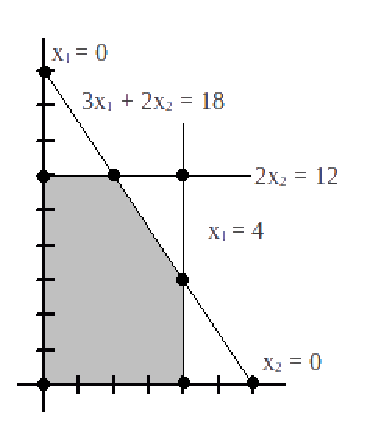
\includegraphics[scale=2.0]{graficos/simplex_graf}
	\captionof{figure}{Representação gráfica de um modelo de programação linear de duas variáveis}
	\label{img:simplex_grafico}
\end{center}

Onde cada reta representa uma restrição do modelo, e a área cinza representa a região viável, ou seja, nessa área estão contidas os valores viáveis de $x_{1}$ e $x_{2}$ para a maximização do lucro.

Os métodos para resolução de problemas de programação linear buscam esses valores de $x_{1}$ e $x_{2}$  para a determinação da solução ótima.

\section{Aplicações utilizando programação linear}
Um problema de programação linear, como já dito anteriormente, busca um resultado ótimo sujeito a restrições, com utilização em diversas áreas.

A programação linear se aplica na área da saúde, como demonstrado por \citeonline{Alterovitz-saude} em seu trabalho. Em um determinado tipo de tratamento de câncer são inseridos cateteres na área afetada para introduzir o medicamento necessário, porém o medicamento acaba afetando células saudáveis além das cancerígenas. Como os problemas de programação linear podem ser resolvidos como problemas determinísticos e com solução exata, \citeonline{Alterovitz-saude} propõe a formulação de um problema de otimização para determinar o tempo de permanência dos cateteres, minimizando os desvios em relação a quantidade da dose necessitada pelo paciente através da minimização de custos atribuídos. Nos testes realizados, foi obtida uma melhoria nos desvios em relação a quantidade da dose necessitada pelo paciente mas clinicamente os resultados obtidos não mostraram uma vantagem significativa em relação ao método atualmente utilizado.

Em \citeonline{Moreira2003Saude} modelos de programação linear foram desenvolvidos para duas aplicações relacionadas a área da saúde. Em um dos modelos busca-se a formulação de uma dieta com custo mínimo, considerando as restrições alimentares e os nutrientes essenciais em uma dieta. Um segundo modelo visa analisar intervenções médicas que buscam maximizar os anos de vida de pacientes considerando uma população, como restrições são utilizados os custos e o número de visitas médicas. Para a resolução dos modelos foi utilizado o método simplex. O autor considerou a programação linear como um instrumento útil na tomada de decisões na área da saúde, considerando a importância da substituição de métodos tradicionais baseados no bom senso e tentativa de acerto por métodos com soluções otimizadas.

Nos trabalhos de \citeonline{Alterovitz-saude} e \citeonline{Moreira2003Saude} foi exemplificado como a programação pode ser útil e importante na área da saúde. No primeiro trabalho apesar de não demonstrar uma melhoria no resultado geral, foi comprovada a equivalência dos resultados com o método probabilístico atualmente utilizado. Em \citeonline{Moreira2003Saude} apesar dos dados utilizados serem reduzidos e uma dieta real possuir mais restrições que as propostas no trabalho, o autor demonstrou a aplicabilidade da programação linear em duas situações da área da saúde.

Em \citeonline{Possami2011Logistica} a programação linear foi utilizada na resolução de um problema abrangendo o transporte, processamento e estocagem de fumo, buscando como objetivo a minimização dos custos. O modelo proposto foi composto por 650 variáveis e 150 restrições. A partir do resultado obtido foi possível determinar parâmetros desde o transporte da matéria bruta, estocagem até a venda do produto.

Dentre as aplicações mais conhecidas da programação linear, encontram-se os problemas de planejamento de produção e controle de estoque, assuntos relacionados a engenharia de produção, como no trabalho de \citeonline{Possami2011Logistica}. A partir desse trabalho tem-se o exemplo de como os resultados extraídos de um modelo de programação linear podem ser determinantes no sucesso de um processo de produção.

Em seu trabalho \citeonline{Krukoski2010Economia} porpõe a utlização da programação linear na economia. Considerando que os investimentos em ações estão cada vez mais acessíveis para pequenos investidores, o autor propõe um modelo de programação linear na determinação de uma operação de compra ou venda que maximize o lucro e baseando-se também nos riscos. Os resultados obtidos em sua maioria foram positivos e lucrativos, apesar de, de acordo com o autor, algumas operações obtidas nos resultados serem pouco aplicáveis se comparadas as atitudes rotineiras dos investidores.

No trabalho proposto por \cite{Krukoski2010Economia} foi apresentada uma aplicação que pode auxiliar na tomada de decisões na área da economia. Os bons resultados mostram que a programação linear, como método determinístico, pode ser empregada mesmo em problemas que estão mais relacionados a métodos probabilísticos, como é o caso dos investimentos em ações.

A programação linear além de estar presente, é fundamental em diversas áreas, tornando-se uma ferramenta de apoio a decisão e contribuindo para o sucesso de projetos nas áreas em que se aplica.

\section{Métodos de Classificação}
Em problemas de classificação, dado um conjunto de dados de treinamento onde cada subconjunto pertence a uma entre \textit{n} classes, o objetivo é que dada uma instância o método de classificação retorne a qual das \textit{n} classes essa instância pertence. A seguir são apresentados alguns dos métodos mais citados na literatura. 

\subsection{\it Support Vector Machines}
\textit{Support Vector Machines} (SVM) ou Máquinas de vetores de suporte têm a capacidade de gerar classificadores na etapa de treinamento e de classificar os dados na etapa de teste de acordo com os classificadores gerados. Considerando um problema de classificação com duas classes, uma SVM irá determinar um plano que separe os pontos dessas duas classe, de forma que a distância entre o hiperplano e os pontos seja a máxima possível. Os pontos de cada classe utilizados como referência são denominados vetores de suporte.
No caso de conjuntos linearmente inseparáveis, é utilizada um função denominada Kernel. Essa função é responsável por elevar a dimensão espacial a fim de que os pontos se tornem linearmente separáveis. Portanto para a obtenção de um classificador utilizando SVM é necessária a escolha de uma função kernel e os parâmetros dessa função. Essa escolha influencia diretamente no desempenho do classificador\cite{Gunn98SVM}\cite{Reffson02SVM}.

No caso em que o número de classes é maior que dois, duas abordagens podem ser utilizadas com as SVM \cite{Lorena03SVM}:
\begin{itemize}
\item{Um contra todos: }Nessa abordagem, para \textit{k} padrões são geradas \textit{k} SVM. Na criação das SVM, é gerado um hiperplano que separa 1 padrão dos \textit{k}-1 padrões. Na determinação do padrão de uma instância x, o padrão é aquele que, entre as \textit{k} SVM obteve mais valores de x do lado do hiperplano onde se encontrava o padrão separado dos demais.  
\item{Todos contra um: }Nessa abordagem os padrões são agrupados em pares e uma SVM é gerada para cada par. Um esquema de votação deve ser utilizado para determinar o padrão de uma instância, que deve ser analisada a partir de cada SVM e cada SVM retorna uma classe possível. A classe que obtiver mais pontos da instância é a classe atribuída.
\end{itemize}

\subsection{\it Naive Bayes}
Na metodologia \textit{Naive Bayes} as características do dado a ser classificado são analisadas de forma independente. O vetor de características é formado pela número de vezes que cada característica ocorre no dado caracterizado. A probabilidade de uma instância pertencer a um determinado padrão é dada por uma probabilidade inicial, baseada na quantidade total de dados, e pelas probabilidades das ocorrências das características \cite{McCallum98Bayes}\cite{Langley92Bayes}. %Essa abordagem é mais comumente utilizada na área de mineração de dados, onde dada uma palavra busca-se o melhor texto baseado na quantidade de vezes que a palavra aparece da palavra no textos utilizados no treinamento% \

\subsection{\textit{k}- nearest neighbor}
Nesse método a classificação é feita pela similaridade da instância a ser classificada com um dado ou vetor utilizado no treinamento, a classe do dado utilizado no treinamento é então atribuída a instância com padrão inicialmente desconhecido. As etapas desse método consistem em utilizar um parâmetro para medir a semelhança ou a distância do dado a ser classificado em relação a cada um dos dados utilizados no treinamento. Os \textit{k} vetores mais similares ou mais próximos são selecionados e entre o padrão mais frequente é atribuído ao dado inicialmente desconhecido. Apesar de ser considerado um método simples, sua dificuldade está em definir os parâmetros ou a métrica que definirá a semelhança ou distância entre os dados\cite{Chagas09KNN}.

\subsection{Redes Neurais Artificias}
Em seu trabalho  \citeonline{Morais2010RNA} define Redes Neurais Artificiais (RNA) como sistemas paralelos e distribuídos compostos por unidades de processamento simples (neurônios) interligadas por conexões, esses neurônios calculam determinadas funções matemáticas. Na fase de treinamento ou aprendizagem "um conjunto de exemplos é apresentado a rede que extrai automaticamente características necessárias para representar a informação fornecida" \cite{Morais2010RNA}.
Uma rede neural pode receber como entrada, na etapa de treinamento, um conjunto de vetores com seus respectivos padrões. Ao submeter como entrada um vetor com padrão desconhecido a rede neural deve classificar esse vetor. A vantagem desse método é que uma rede pode construir fronteiras não lineares entre padrões, o que pode ser muito vantajoso em problemas complexos de classificação. Existem vários modelos de redes neurais que possibilitam o reconhecimento de padrões, entre eles: Perceptron de Camada Simples, Perceptron de Múltiplas e Redes de Kohonen \cite{ZubenRNA2}.

\section{Aplicações em classificação de dados}
Em seu trabalho \citeonline{Reffson02SVM} busca o classificação de impressões digitais em 5 classes. Esse tipo de classificação tem o propósito de gerenciar grandes bancos de dados de impressões digitais e acelerar o processo de identificação. Foi utilizado um banco contendo 4000 imagens igualmente distribuídas entre as cinco classes. O autor dividiu o banco em dois grupos, utilizando um para treinamento e outro para teste. Após a extração das características das imagens, Máquinas de Vetores de Suporte foram utilizadas na classificação. Na abordagem todos contra um foi obtida uma média de precisão de 91,18\%, já na abordagem um contra todos a precisão na classificação das impressões foi de 90,43\%.

\citeonline{Chagas09KNN} apresentou uma técnica para a classificação de textos, uma atividade importante em aplicações como bibliotecas digitais e em outras que em geral buscam a organização de documentos disponíveis no formato digital. O autor propôs variações no método \textit{k near neighbor} a fim de  aprimorar a escolha dos textos, utilizados no treinamento, mais próximos ao texto que precisa ser classificado. Nos testes feitos com três coleções de textos, as médias de acertos na classificação obtidas foram acima de 90\% em duas coleções, e próxima a 70\% na terceira.

No trabalho de \citeonline{sbai2003RNALaranjas} uma rede neural artificial foi utilizada na classificação de laranjas através de imagens. Os autores consideraram que apesar da automação de muitos setores industriais, em um sistema de produção, as frutas consideradas boas, são selecionadas através de inspeção visual humana. A principal característica utilizada foi a cor, que pode classificar a fruta em cinco padrões. No trabalho ficou comprovada a aplicabilidade do método para o domínio proposto que era classificar as frutas de acordo com a cor.

\section{Métodos de validação do modelo}
Um modelo de classificação pode ser verificado em relação a sua acurácia a partir de um conjunto de dados ou a sua performance em relação a outros métodos classificadores. Algumas técnicas utilizadas com esse intuito serão apresentadas a seguir. No presente trabalho a técnica Cross Validation é utilizada com o objetivo de verificar a acurácia, nesse caso, da metodologia utilizada na classificação de dados.

A seguir são apresentadas as três técnicas mais comumente encontradas na bibliografia com suas ventagens e desvantagens:

\subsection{\textit{Handout}}
Esse é um método simples, onde os dados são divididos em 2 grupos mutuamente exclusivos, sendo um grupo utilizado para treino e o outro para teste. Em geral 2/3 dos dados são utilizados no treinamento e 1/3 na etapa de testes. Os dois grupos devem conter dados suficientes de todos os padrões, nesse caso, suficientes para que o resultado final não seja comprometido pela falta de dados no grupo da etapa de treino e nem no grupo de testes. Apesar de ser um método de fácil implementação, a divisão entre conjunto de treinamento e teste deve ser bem estudada de forma que todos os padrões estejam bem representados nos dois grupos, por isso é um método recomendável quando o conjunto de dados possui um grande número de representações de cada padrão \cite{Kohavi95Cross} \cite{Baldisserotto05Validacao}.

\subsection {\textit{Cross Validation}}
Nesse método, o conjunto de dados também é dividido em conjunto de treinamento e de teste, porém esses dois grupos variam a cada rodada de teste. O tipo de \textit{cross validation} mais comumente utilizado é o \textit{k-fold cross validation}, onde os dados são divididos em k conjuntos mutuamente exclusivos e as etapas de treinamento e teste são realizadas k vezes, de forma que a cada rodada um conjunto diferente é utilizado como teste e os outros k-1 conjuntos são utilizados para treinamento. Esse método é recomendável quando o conjunto de dados não é tão grande, pois não existe uma  preocupação de quais dados separar para teste e quais separar para validação, já que ao final da execução do método todos o dados terão participado dos conjuntos de validação e teste \cite{Kohavi95Cross} \cite{Baldisserotto05Validacao}.

\subsection{\textit{Leave-one-out}}
Nessa técnica, do conjunto com o número total de dados n, são realizadas n rodadas de treinamento e teste, sendo que a cada rodada n-1 dados são utilizados para teste e o dados restantes são utilizados para treinamento. Pelas suas características, esse é um método recomendável para conjuntos de dados pequenos já que a quantidade de rodadas de treinamento e teste é igual a quantidade de dados o que o torna um método com alto custo computacional \cite{Kohavi95Cross} \cite{Baldisserotto05Validacao}.
